\chapter{Architektura systemu}
\label{Chapter5}

\begin{figure}[H] 
\centering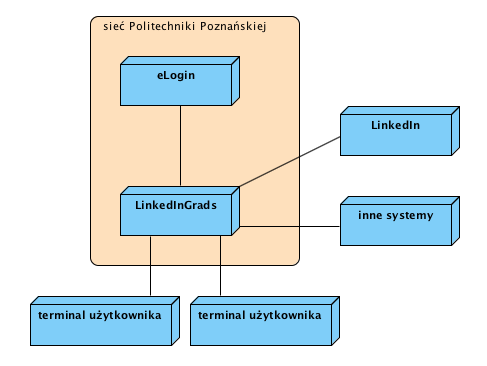
\includegraphics[width=15cm]{figures/image2}
\caption{Architektura systemu LinkedInGrads}\label{rys:use-case-diagram}
\end{figure}

W rozdziale przedstawione zostaną zagadnienia związane z architekturą systemu LinkedInGrads. Ukazane zostaną zastosowane podejścia architektoniczne, podjęte decyzje (razem z ich uzasadnieniami oraz zależnościami), zobrazowany będzie przyjęty schemat bazy danych. W celu lepszego przedstawienia tematu architektury, ze względu na jego złożoność, w podrozdziale 5.4. Perspektywy architektoniczne wykorzystano model 4+1 Views.

\section{Zastosowane podejście architektoniczne}
\label{Chapter52}

Rozdział dotyczy wzorca projektowego, w oparciu o który zaprojektowano architekturę systemu.

\section{Analiza SWOT}
\label{Chapter53}

Analiza SWOT przyjętego podejścia architektonicznego.

\section{Perspektywy architektoniczne}
\label{Chapter54}

\subsection{Perspektywa fizyczna}

Rysunek wraz z opisem.

\subsection{Perspektywa logiczna}

Rysunek wraz z opisem.

This view of the architecture addresses the functional requirements of the system, in other words, what the system should do for its end users. It is an abstraction of the design model and identifies major design packages, subsystems, and classes.


\subsection{Perspektywa implemetancyjna}

Rysunek wraz z opisem. Można tutaj też umieścić perspektywę kodu.

This view describes the organization of static software modules (source code, data files, components, executables, and other accompanying artifacts) in the development environment in terms of packaging and layering and in terms of configuration management (ownership, release strategy, and so on). It addresses the issues of ease of development, management of software assets, reuse, subcontracting, and off-the-shelf components.


\subsection{Perspektywa procesu (równoległości)}

Rysunek wraz z opisem.

This view addresses the concurrent aspects of the system at runtime—tasks, threads, or processes as well as their interactions. It addresses issues such as concurrency and parallelism, system start-up and shutdown, fault tolerance, and object distribution. It deals with issues such as deadlock, response time, throughput, and isolation of functions and faults. It is concerned with scalability.
Examples are a flight management process, flight plan entry processes, and an airspace management process.


\section{Decyzje projektowe}
\label{Chapter55}

Tutaj piszemy o decyzjach projektowych, związkach pomiędzy nimi oraz innych związanych sprawach.

\section{Wykorzystane technologie}
\label{Chapter56}

Opis wykorzystywanych technologii (COTS).

\section{Schemat bazy danych}
\label{Chapter57}

Schemat bazy danych, ze względu na objętość, można umieścić w którymś dodatku.